\documentclass[a4paper, 11pt]{article}
\usepackage[utf8]{inputenc}

\usepackage[french]{babel}
\usepackage{graphicx} 
\usepackage{hyperref}
\usepackage{xcolor}
\usepackage{listings}
\usepackage{enumitem}
\usepackage{amsmath} 

\usepackage{amsfonts}
\usepackage{hyperref}
\usepackage{array,booktabs,makecell,multirow}
\usepackage{siunitx}
\usepackage[left=2cm ,right=2cm ,bottom=2cm,top=2cm]{geometry}
\usepackage{algorithm}
\usepackage{algorithmic}
\usepackage{pifont}
\usepackage{xcolor}
\usepackage{subcaption}

% to display code
\usepackage{minted}
\usemintedstyle{default}
\setminted{fontsize=\scriptsize, baselinestretch=0.5}

\newcommand{\HRule}{\rule{\linewidth}{0.5mm}}

\begin{document}

\begin{titlepage}

\begin{center}

\includegraphics[scale = 0.35]{logo.jpg}\\
\vspace{1cm}
\textsc{\huge University of Liège}\\[1.2cm]
\HRule \\[1cm]
\textsc{\LARGE ELEN0040 : Digital Electronics }\\[1cm]
{\Huge \bfseries Project Report}\\[1.4cm] 
\HRule \\[1cm]
\end{center}
\begin{figure}[H]
    \centering
    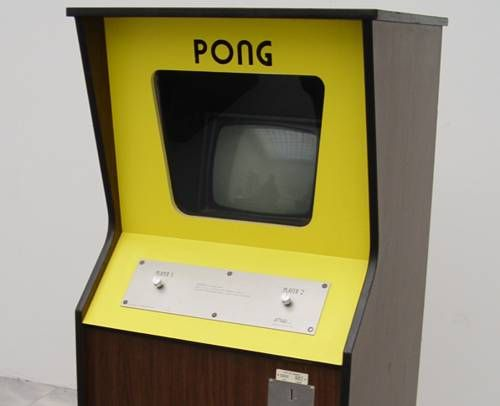
\includegraphics[scale = 0.55]{Ressources/png/pong_image.jpg}
\end{figure}
\begin{minipage}{0.45\linewidth}
      \begin{flushleft} \large
        \emph{Authors : } \\
        Grégoire Hendrix  s214754 \\
        Louis Hogge  s192814 \\
        Arnaud Innaurato  s211234 \\
        Macha Krumm  s212449
      \end{flushleft}
\end{minipage}
\hfill
\begin{minipage}{0.35\linewidth}
      \begin{flushleft} \large
        \emph{Professor : } J-M Redouté \\
        \emph{Teaching Assistants : } A. Fyon \\ \phantom{\emph{Teaching Assistants: }} A. Halin \\ 
        \emph{Year : } 2022-2023 
      \end{flushleft}
\end{minipage}

\end{titlepage}


\newpage

\section{Introduction}

This project aims to implement a simplified version of the game \href{http://www.ponggame.org/}{\textit{pong}} by using a CPLD. The goal is to bounce the ball on the paddle. The simplified version consists of a single paddle that moves horizontally and a ball that moves vertically, the player has the ability to control the movement of the paddle in order to bounce the ball up. When the ball reaches the top, it bounces back in another column, which is drawn randomly. This version of the game was necessary in order to fit our game on this kind of microchips with only 160 logic gates. The game stops when the player fails 3 times to make the ball bounces on the paddle.\\

We chose to use a 5x7 LED matrix where the paddle moves in the row of 7 LEDs and the ball in the column of 5 LEDs. The paddle has a width of 2 LEDs and the ball has a size of only 1 LED.


\section{Hardware}

Here is the electrical schematic of our project:


\begin{figure}[H]
    \centering
    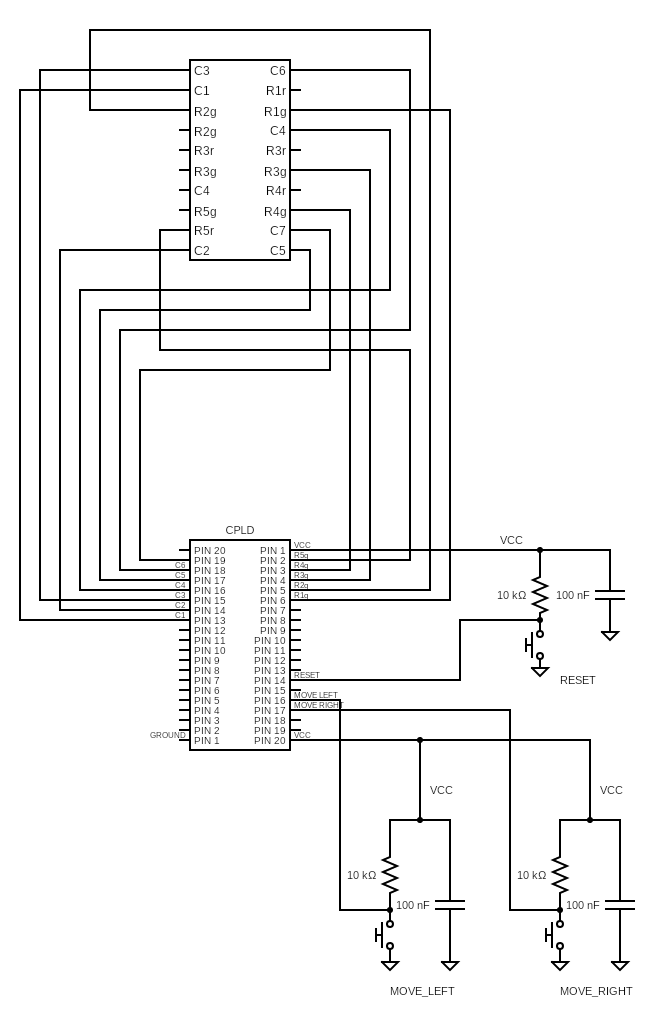
\includegraphics[scale = 0.4]{Ressources/png/circuit.png}
    \caption{Electrical schematics}
    \label{fig:my_label}
\end{figure}

The player needs three buttons to control the game. One to move the paddle to the left, another one to move it to the right and the last one to start/reset the game. Here is the explanation of how they work :  \\
\begin{itemize}

    \item[$\bullet$] \textbf{Move buttons:} The buttons have to be pushed to move the paddle. It means that it detects when \texttt{MOVE\_LEFT} = '0' or if \texttt{MOVE\_RIGHT} = '0'. As represented in the schematic, when a button is pushed, the input voltage is the ground so it is why we have '0'. To make sure that we do not have any voltage bounces, each button is in series with a 10 $k\Omega$ resistance and in parallel with a 100 nF capacitor. \\

    \item[$\bullet$] \textbf{Reset button:} This button has to be pushed to start playing, to play again if you have lost or to reset the game while you are playing. It is also in series with a 10 $k\Omega$ resistance and in parallel with a 100 nF capacitor. It works like the two other buttons : if you push it, the voltage goes to the ground and the input signal \texttt{START} = '0'. When reset button is pressed, the game starts again with 3 lives. \\
\end{itemize}

For the LED matrix, we used a bi-color 5 x 7 LED matrix \href{https://www.kingbrightusa.com/images/catalog/SPEC/TBC20-11EGWA.pdf}{(TBC20-11EGWA)}. We used 12 of the 20 pins available. For the 4 first rows, we used the green LEDs and for the last row (the bottom one) we used the red LEDs.

\begin{center}
\begin{tabular}{|c|c|c|}
\hline
\multicolumn{3}{|c|}{LED to chip pin assignment}\\
\hline
Name & pin on the CPLD & location on the chip \\
\hline
Row 1 green & pin 12 & pin 1 \\
\hline
Row 2 green & pin 10 &  pin 2\\
\hline
Row 3 green  & pin 8 &  pin 3\\
\hline
Row 4 green & pin 6 & pin 4\\
\hline
Row 5 red & pin 4 & pin 5\\
\hline
Column 1 & pin 15 & pin 56\\
\hline
Column 2 & pin 13 & pin 58\\
\hline
Column 3 & pin 11 & pin 59\\
\hline
Column 4 & pin 9 & pin 60 \\
\hline
Column 5 & pin 7 & pin 61\\
\hline
Column 6 & pin 5 & pin 62\\
\hline
Column 7 & pin 3 & pin 63\\

\hline
\end{tabular}
\label{table_1}
\end{center}
\section{Main entity and inputs/outputs}

Here is the main entity of our game:

\begin{minted}{vhdl}
entity pong is
    generic(
        -- Constants
        SCREEN_WIDTH: integer := 7;
        SCREEN_HEIGHT: integer := 5;
        PADDLE_WIDTH: integer := 2;
        PADDLE_Y: integer := 0;
        NUMBER_LIVES: integer := 3);
    Port(
        -- Input signals
        CLK_SLOW: in STD_LOGIC;
        CLK_FAST: in STD_LOGIC;

        MOVE_LEFT: in STD_LOGIC;
        MOVE_RIGHT: in STD_LOGIC;

        START: in STD_LOGIC;

        -- Output signals
        LED_ROW: out STD_LOGIC_VECTOR(SCREEN_HEIGHT - 1 downto 0);
        LED_COL: out STD_LOGIC_VECTOR(SCREEN_WIDTH - 1 downto 0);
        
        LED_LIVES: out STD_LOGIC_VECTOR(NUMBER_LIVES - 1 downto 0));
end pong;
\end{minted}

\subsection{Constants}
\begin{itemize}
        \item[-] \texttt{SCREEN\_WIDTH} : equals to the LED matrix's width (7)
        
        \item[-] \texttt{SCREEN\_HEIGHT} : equals to the LED matrix's height (5)
        
        \item[-] \texttt{PADDLE\_WIDTH} : the paddle's size has been defined to 2 in this game
        
        \item[-] \texttt{PADDLE\_Y} : the paddle stays at the bottom so its position is equal to 0
        
        \item[-] \texttt{LIVES} : the number of lives has been chosen to be equal to 3
\end{itemize}
\subsection{Inputs}
\begin{itemize}
    \item[-] \texttt{CLOCK\_SLOW} : the slowest clock from the CPLD
    \item[-] \texttt{CLOCK\_FAST} : the fastest clock from the CPLD
    \item[-]\texttt{MOVE\_LEFT} : button that moves the paddle one LED to the left
    \item[-] \texttt{MOVE\_RIGHT} : button that moves the paddle one LED to the right
    \item[-] \texttt{START} : button that starts or restarts the game with 3 lives
\end{itemize}
\subsection{Outputs}
\begin{itemize}
    \item[-] \texttt{LED\_ROW} : logic vector which contains the lines of the LED matrix
    \item[-] \texttt{LED\_COL} : logic vector which contains the columns of the LED matrix
    \item[-] \texttt{LIVES} : logic vector that contains the number of remaining lives
\end{itemize}
\section{Game structure}

This schematic explains visually the different steps of the game operations:

\begin{figure}[H]
    \centering
    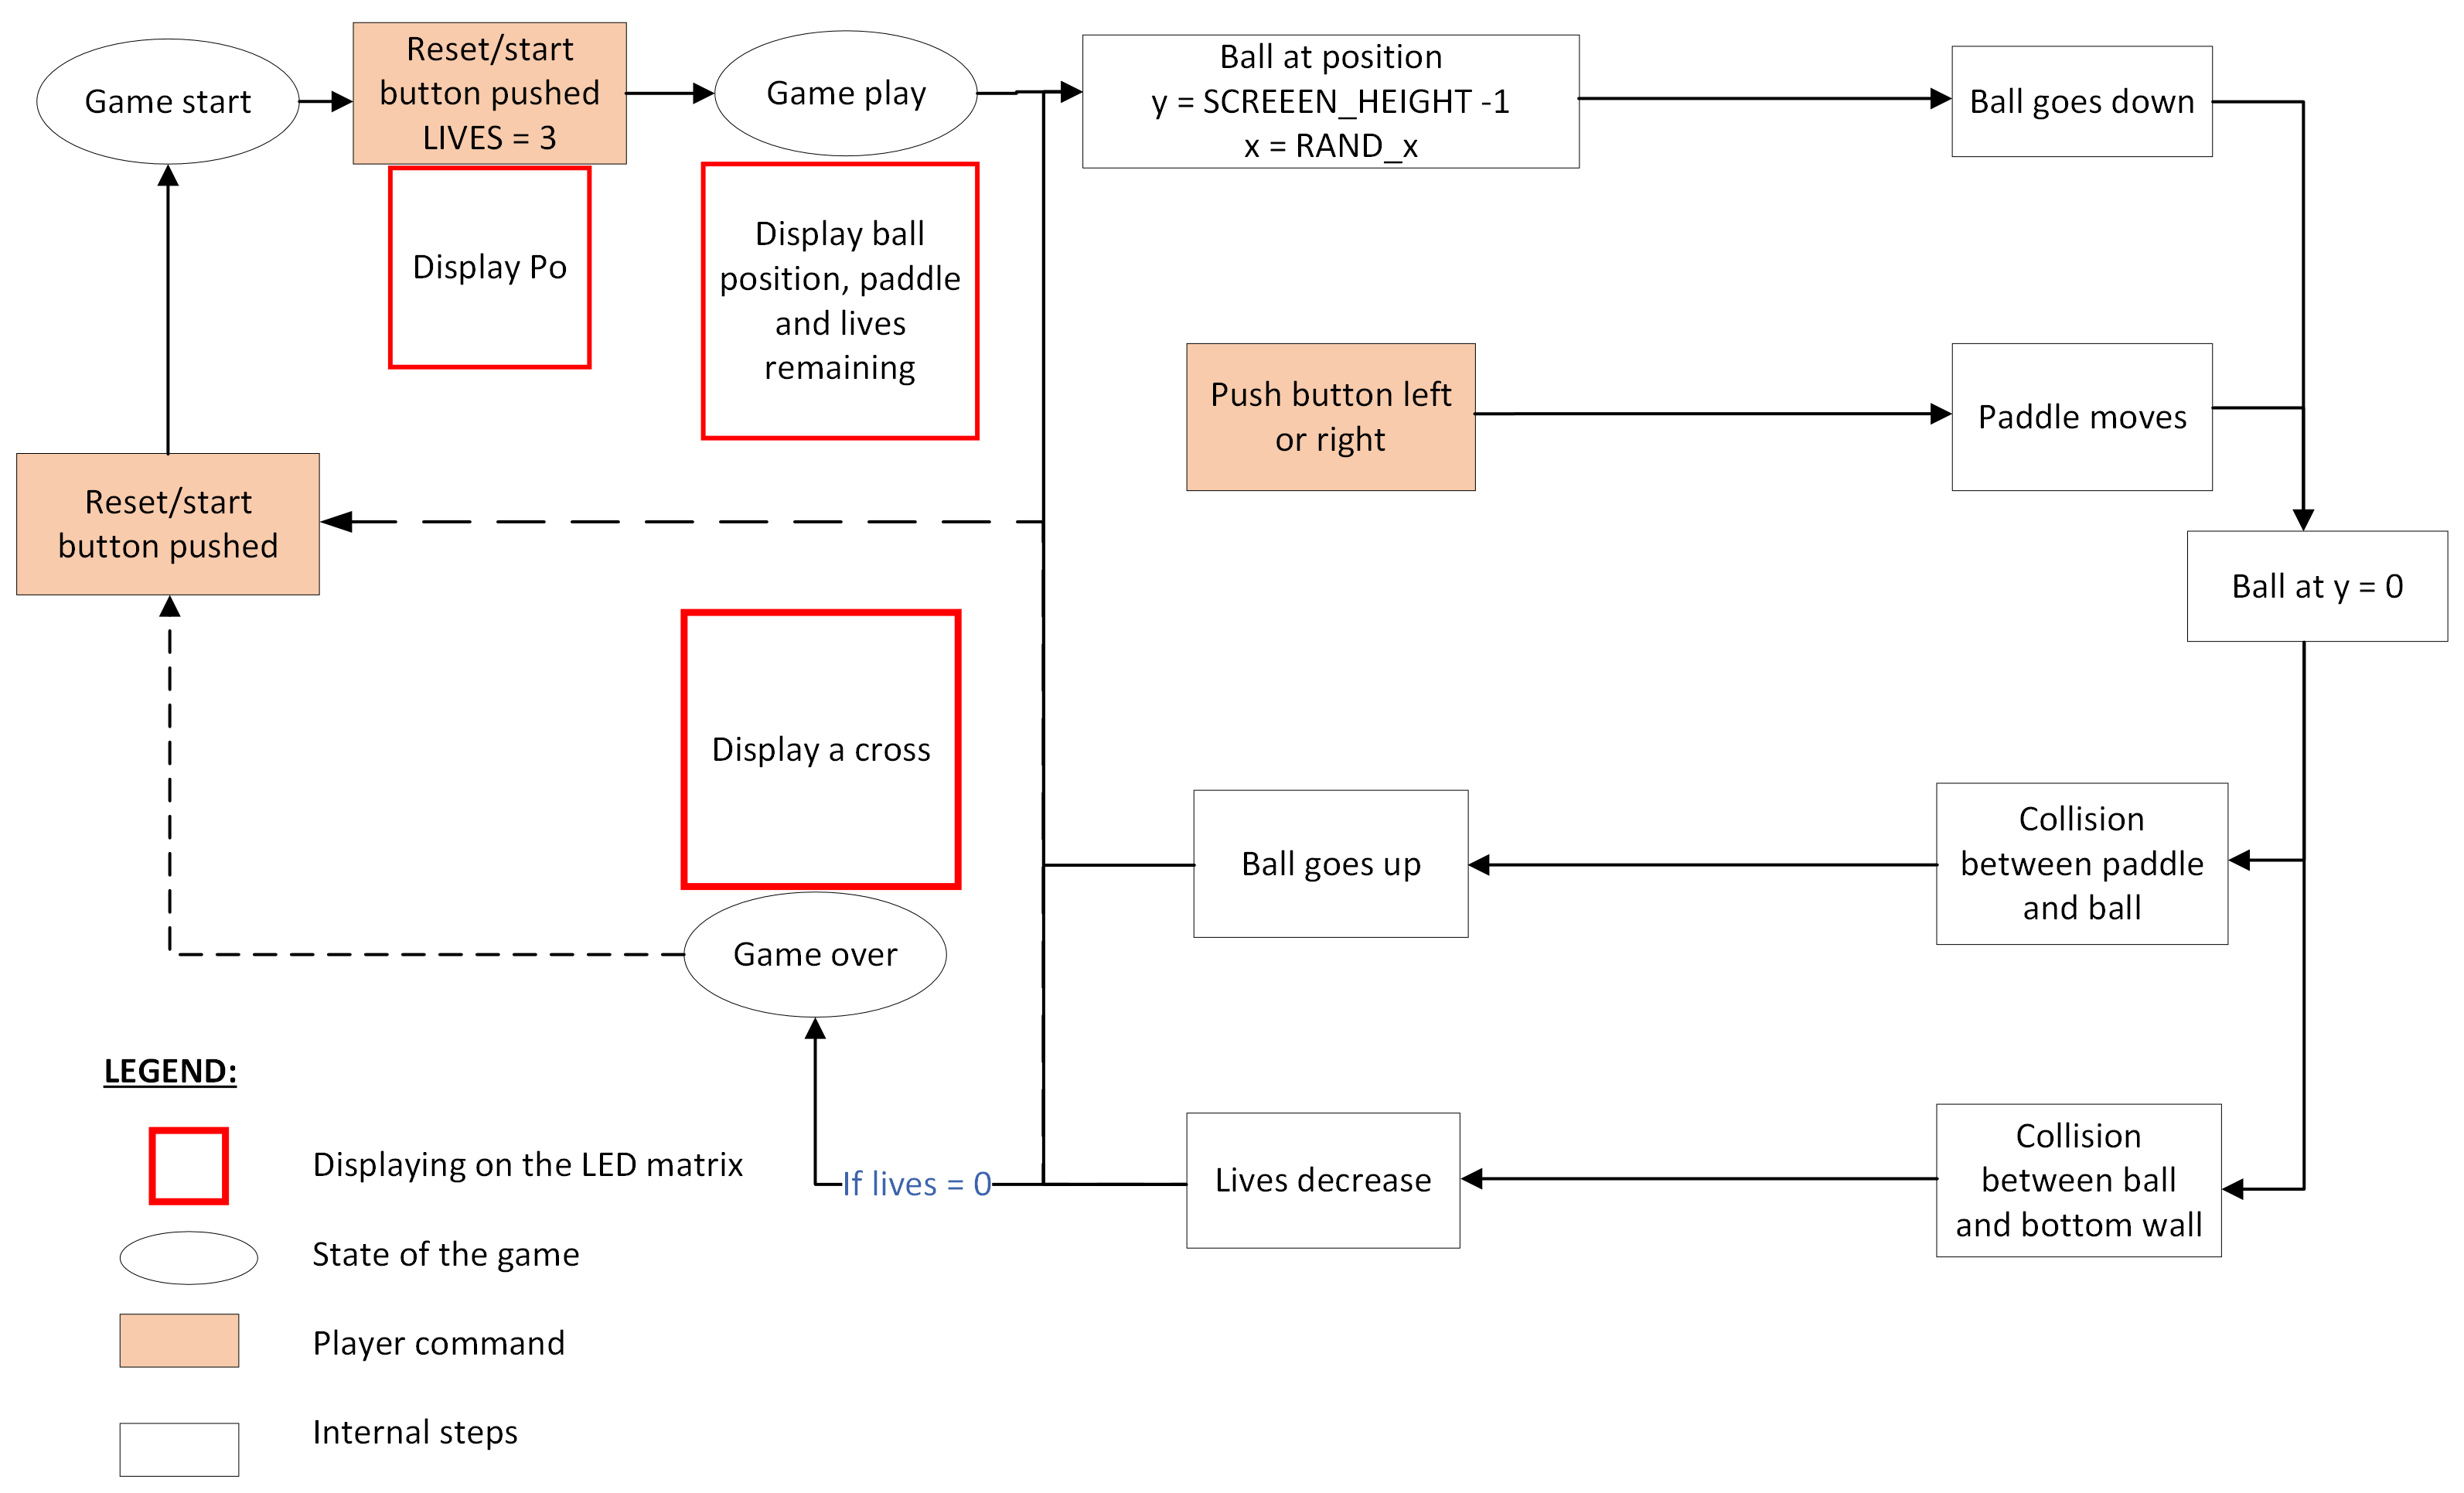
\includegraphics[scale = 0.25]{Ressources/png/Dessin.png}
    \caption{Structure of the game}
    \label{fig_3}
\end{figure}
\section{Code structure} 
NB : All the code is given in the section \ref{Code}.

\begin{itemize}
    \item[$\bullet$] \textbf{Variables:}
    \begin{itemize}
        \item[-] \texttt{BALL\_X} : the horizontal position of the ball, which can take values between 0 and 6\\
        
        \item[-] \texttt{BALL\_Y}  : the vertical position of the ball, which can take values between 0 and 4\\
        
        \item[-] \texttt{PADDLE\_X} : the horizontal position of the left corner of the paddle, which can take values between 0 and 5\\
        
        \item[-] \texttt{RAND\_X} : a number generated to randomly determine the position of the ball when it hits the top wall\\
        
        \item[-] \texttt{BALL\_DIRECTION} : direction of the ball's movement, can be \textit{up} or \textit{down}\\
        
        \item[-] \texttt{GAME\_STATE} : indicates the state of the game, it can be $game\_start$ (before the start of a game), $game\_play$ (when a game is in progress) or $game\_over$ (when you have lost) \\
        
        \item[-] \texttt{LIVES} : are decremented when the ball hits the bottom wall, take values from 3 to 0
        
        \begin{figure}[H]
        \centering
        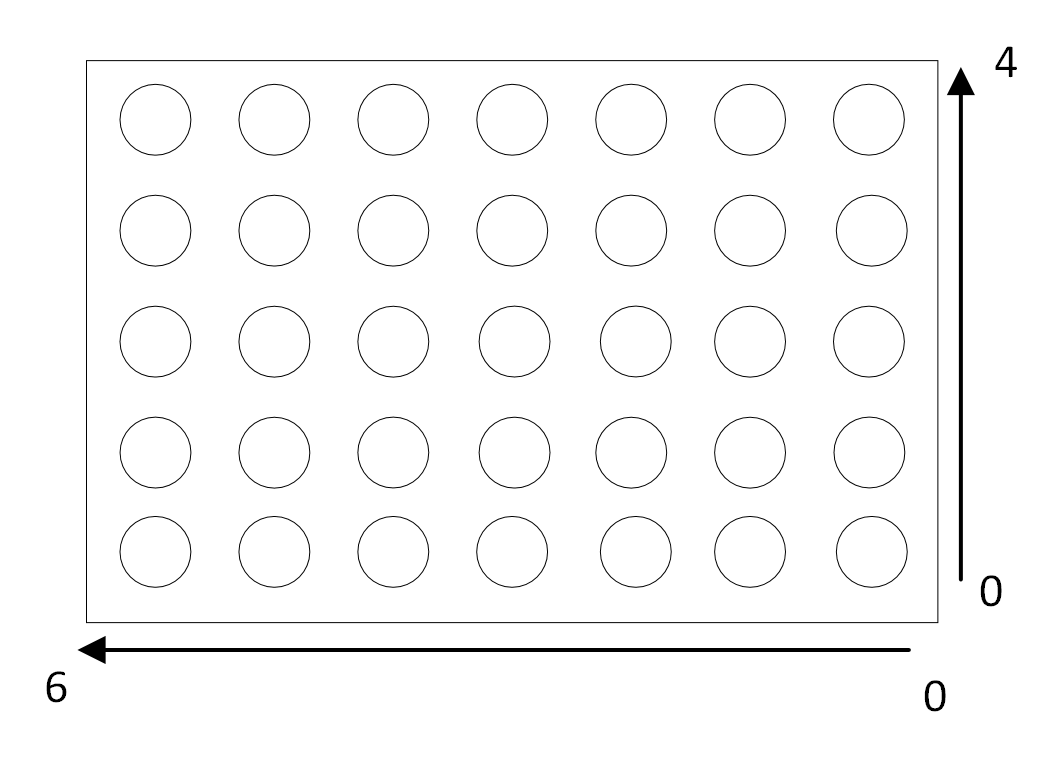
\includegraphics[scale = 0.25]{Ressources/png/Dessin1.png}
        \caption{Visualization of the coordinates chosen for the LED matrix}
\end{figure}
        
    \end{itemize}
    \item[$\bullet$] \textbf{Processes:} 
    \begin{itemize}
        \item[-] \textit{Random} : generates a number to randomly determine the position of the ball when it hits the top wall. It is triggered at the rising edge of the \texttt{CLK\_FAST}. It goes from 0 to 6 and when it's value is equal to 6, it returns to 0. The computation of the next value of our ball position on the top wall is only done triggering the \texttt{CLK\_SLOW} which assure that our number is random.\\
        
        \item[-] \textit{paddle movement} : if one of the button (left or right) is pressed, we check if the paddle can go in the desired direction. If so, the paddle moves in the direction wanted. It is triggered by the \texttt{CLK\_SLOW}.\\
        
        \item[-] \textit{ball movement} : Triggered by the \texttt{CLK\_SLOW}, this process handles the movement of the ball and the collisions with the paddle. There are 4 types of collisions in this implementation : 
        \begin{itemize}
            \item[-] paddle collision : if the ball is at the bottom wall, we check if its horizontal position corresponds to one of the two points of the paddle. If it collides, the ball will go up by changing \texttt{BALL\_DIRECTION} to \textit{up}\\
            
            \item[-] bottom collision : if the ball is at the bottom wall but there is not a collision with the paddle, \texttt{LIVES} is decremented and the ball will start at a random position at the top wall\\

            \item[-] top collision : when the ball is at the top, its position is updated with random position x and the ball will start going down from that new position \\

            \item[-] no collision : handles the cases when the ball is between the top and the bottom wall. It checks the \texttt{BALL\_DIRECTION} and increments \texttt{BALL\_Y} if it is \textit{up} or decrements it if it is \textit{down}
        \end{itemize}
        
        \hangindent=\labelwidth \hangafter=0 When the reset button is pressed, this process is responsible of giving a new random \hangindent=\labelwidth \hangafter=0 horizontal position at the top row.
        
        \item[-] \textit{display} : Before the game starts, '\textbf{P}' is shown on the LED matrix. When the game is playing, it displays the correct LEDs and when the game is over, it displays a cross on the matrix. It is triggered by the \texttt{CLK\_FAST} to have the correct fluency for the LEDs.\\

        \item[-] \textit{state management} : manages the states of the games. When the start button is pressed, it starts the game by putting \texttt{GAME\_STATE} at $game\_play$. The game goes on until there are no more lives remaining. Once the game is done,  \texttt{GAME\_STATE} is set at $game\_over$. 
    \end{itemize}
\end{itemize}

\section{Simulation}
This section shows a simulation of our game done in ModelSim. It shows the proper functioning of \texttt{LIVES}. The \texttt{CLK\_SLOW} is set to 10ns and the \texttt{CLK\_FAST} to 0.1ns to correctly display the LEDs. To simulate the movement of the paddle, the clock of \texttt{MOVE\_LEFT} is set at 0.5 sec and the clock of \texttt{MOVE\_RIGHT} at 0.4 sec. \texttt{GAME\_STATE} is at game\_play. The simulation lasts 3 seconds. It behaves like expected. \\

\begin{figure}[H]
    \centering
    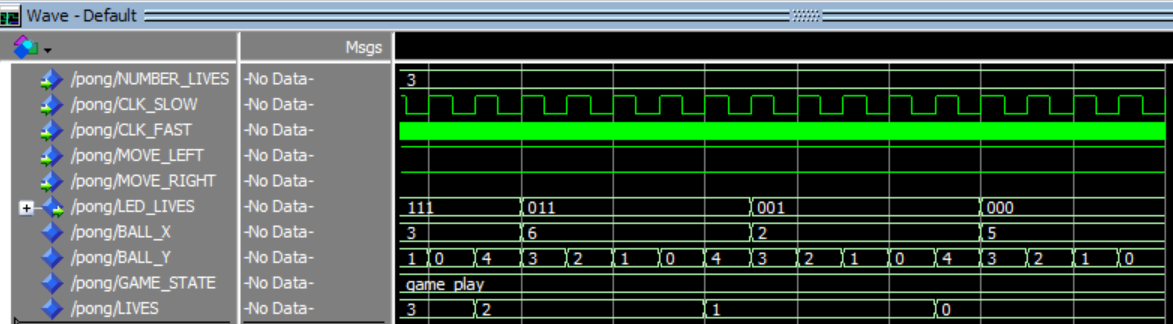
\includegraphics[scale = 0.3]{Ressources/png/simu.png}
    \caption{Simulation}
    \label{fig_2}
\end{figure}

It shows that \texttt{LIVES} decreases and that \texttt{LED\_LIVES} is correctly decremented. The \texttt{LIVES} go correctly from 3 to 0 and are decremented when \texttt{BALL\_Y} is at 0. \texttt{BALL\_X} is a random number and \texttt{BALL\_Y} is between 0 and 4. 
\section{Code} \label{Code}
The code we implemented uses 94 logic gates of our chip , which corresponds to $59\% $ of its capacity. We use 20 pins of the 54 available:
\begin{minted}{vhdl}
library IEEE;
use IEEE.STD_LOGIC_1164.ALL;
use IEEE.STD_LOGIC_UNSIGNED.ALL;

-- Pong game
entity pong is
    generic(
	-- Constants
        SCREEN_WIDTH: integer := 7;
        SCREEN_HEIGHT: integer := 5;
        PADDLE_WIDTH: integer := 2;
        PADDLE_Y: integer := 0;
	NUMBER_LIVES: integer := 3);
    Port(
        -- Input signals
        CLK_SLOW: in STD_LOGIC;
        CLK_FAST: in STD_LOGIC;

        MOVE_LEFT: in STD_LOGIC;
        MOVE_RIGHT: in STD_LOGIC;

        START: in STD_LOGIC;

        -- Output signals
        LED_ROW: out STD_LOGIC_VECTOR(SCREEN_HEIGHT - 1 downto 0);
        LED_COL: out STD_LOGIC_VECTOR(SCREEN_WIDTH - 1 downto 0);

	LED_LIVES: out STD_LOGIC_VECTOR(NUMBER_LIVES - 1 downto 0));
end pong;

architecture behavioral of pong is
    -- Internal signals for game logic
    signal BALL_X: integer range 0 to SCREEN_WIDTH - 1 := 0;
    signal BALL_Y: integer range 0 to SCREEN_HEIGHT - 1 := SCREEN_HEIGHT - 1;

    signal PADDLE_X: integer range 0 to SCREEN_WIDTH - PADDLE_WIDTH := 0;

    signal RAND_X: integer range 0 to SCREEN_WIDTH - 1 := 0;

    type direction is (up, down);
    signal BALL_DIRECTION: direction := down;

    type state is (game_start, game_play, game_over);
    signal GAME_STATE: state := game_start;

    signal LIVES: integer range 0 to NUMBER_LIVES := NUMBER_LIVES;
	 
begin
    -- Random number generator process
    random: process(CLK_FAST)
    begin
        if rising_edge(CLK_FAST) then
            -- Playing the game
            if GAME_STATE = game_play then
                if(RAND_X = SCREEN_WIDTH - 1) then
                    RAND_X <= 0;
                else 
                    RAND_X <= RAND_X + 1;
                end if; 
            end if;
        end if;
    end process random;
    
    
    -- Paddle movement process
    paddle_movement: process(CLK_SLOW)
    begin
        if rising_edge(CLK_SLOW) then
            -- Playing the game
            if GAME_STATE = game_play then
                if MOVE_LEFT = '0' then
                    if not (PADDLE_X = 0) then
                        PADDLE_X <= PADDLE_X - 1;
                    end if;
                elsif MOVE_RIGHT = '0' then
                    if not (PADDLE_X = SCREEN_WIDTH - PADDLE_WIDTH) then
                        PADDLE_X <= PADDLE_X + 1;
                    end if;
                end if;
            end if;
        end if;
    end process paddle_movement;

    -- Ball movement process
    ball_movement: process(CLK_SLOW)
    begin
        if rising_edge(CLK_SLOW) then
            -- Playing the game
            if GAME_STATE = game_play then
                if BALL_Y = 0 then
                    -- Paddle colision
                    if BALL_X = PADDLE_X or BALL_X = PADDLE_X+1 then
                        BALL_DIRECTION <= up;
                        BALL_Y <= BALL_Y + 1;
                    -- Bottom colision
                    else
                        LIVES <= LIVES - 1;
                        BALL_X <= RAND_X;
                        BALL_Y <= SCREEN_HEIGHT - 1;
                    end if;
                -- Top colision
                elsif BALL_Y = SCREEN_HEIGHT then
                    BALL_DIRECTION <= down;
                    BALL_X <= RAND_X;
                    BALL_Y <= BALL_Y - 1;
                -- No colision
                else
                    case BALL_DIRECTION is
                        when up =>
                            BALL_Y <= BALL_Y + 1;
                        when down =>
                            BALL_Y <= BALL_Y - 1;
                    end case;
                end if;
            end if;

            -- Set up the game for restart
            if GAME_STATE = game_start then
                BALL_Y <= SCREEN_HEIGHT - 1;
                LIVES <= NUMBER_LIVES;
            end if;
	end if;
    end process ball_movement;

    -- Display process
    display: process(CLK_FAST)
        -- Counter to display alternatively
        variable COUNTER : integer range 0 to 3 := 0;
    begin
        if rising_edge(CLK_FAST) then
            case GAME_STATE is
                -- Ready to play the game
                when game_start =>
                    -- Initialize control signals to draw "P"
                    if COUNTER = 3 then
                        LED_COL <= "0010000";
                        LED_ROW <= "10000";
                        COUNTER := 0;
                    end if;
                      
                    if COUNTER = 2 then
                        LED_COL <= "0001100";
                        LED_ROW <= "01011";
                    end if;
                      
                    if COUNTER = 1 then
                        LED_COL <= "0010100";
                        LED_ROW <="00011";
                    end if;

                    COUNTER:= COUNTER + 1;
                -- Playing the game
                when game_play =>
                    if LIVES /= 0 then
                        if COUNTER = 3 then
                            -- Paddle display
                            LED_COL <= "0000000"; 
                            LED_ROW <= "11110";

                            -- Set control signals for paddle
                            LED_COL(PADDLE_X) <= '1';
                            LED_COL(PADDLE_X + 1) <= '1'; -- Paddle width is 2

                            COUNTER := 0;
                        else
                            -- Ball display
                            LED_COL <= "0000000"; 
                            LED_ROW <= "11111";

                            -- Set control signals for ball
                            LED_COL(BALL_X) <= '1';
                            LED_ROW(BALL_Y) <= '0';

                            COUNTER := COUNTER + 1;
                        end if;
                    end if;
                -- Game lost  
                when game_over =>
                    -- Initialize control signals to draw a cross
                    if COUNTER = 3 then
                        LED_COL <= "0100010";
                        LED_ROW <= "01110";
                        COUNTER := 0;
                    end if;
                    
                    if COUNTER = 2 then
                        LED_COL <= "0010100";
                        LED_ROW <= "10101";								
                    end if;

                    if COUNTER = 1 then
                        LED_COL <= "0001000";
                        LED_ROW <= "11011";
                    end if;
                    
                    COUNTER := COUNTER + 1;
            end case;
        end if;
    end process display;
	 
    state_management: process(CLK_SLOW)
    begin
        if rising_edge(CLK_SLOW) then
            case GAME_STATE is
            
                -- Ready to play the game
                when game_start =>
                    -- Start the game  
                    if START = '0' then
                        GAME_STATE <= game_play;
                    end if;
                    
                -- Playing the game
                when game_play =>  
                    -- Lives management
                    for i in 0 to NUMBER_LIVES - 1 loop
                        if i < LIVES then
                            LED_LIVES(i) <= '1';
                        else
                            LED_LIVES(i) <= '0';
                        end if;
                    end loop;
                    
                    -- Game lost
                    if LIVES = 0 then
                        GAME_STATE <= game_over;
                    end if;

                    -- Reset the game
                    if START = '0' then
                        GAME_STATE <= game_start; 
                    end if;
     
               -- Game lost
               when game_over =>
                    -- Reset the game
                    if START = '0' then
                        GAME_STATE <= game_start;
                    end if;
            end case;
        end if;
    end process state_management;
end architecture behavioral;

\end{minted}

\newpage
\section{Pin Planner}
\begin{figure}[h!]
  \centering
  \begin{subfigure}{0.45\linewidth}
    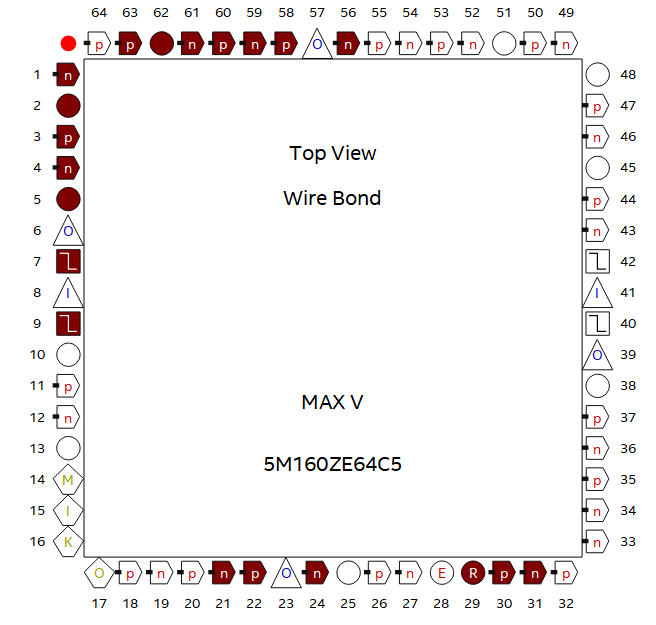
\includegraphics[width=\linewidth]{Ressources/png/pinPlanner.png}
    \caption{}
  \end{subfigure}
  \begin{subfigure}{0.45\linewidth}
    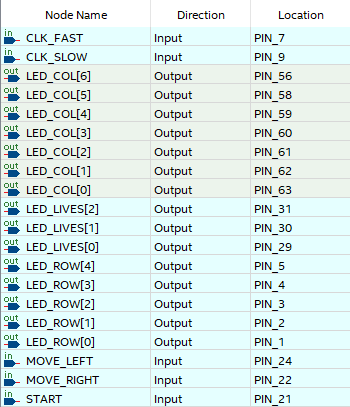
\includegraphics[width=\linewidth]{Ressources/png/pins.png}
    \caption{}
  \end{subfigure}
  \caption{Pin planner}
  \label{Pin planner}
\end{figure}




\end{document}
